%% bare_conf.tex
%% V1.3
%% 2007/01/11
%% by Michael Shell
%% See:
%% http://www.michaelshell.org/
%% for current contact information.
%%
%% This is a skeleton file demonstrating the use of IEEEtran.cls
%% (requires IEEEtran.cls version 1.7 or later) with an IEEE conference paper.
%%
%% Support sites:
%% http://www.michaelshell.org/tex/ieeetran/
%% http://www.ctan.org/tex-archive/macros/latex/contrib/IEEEtran/
%% and
%% http://www.ieee.org/

%%*************************************************************************
%% Legal Notice:
%% This code is offered as-is without any warranty either expressed or
%% implied; without even the implied warranty of MERCHANTABILITY or
%% FITNESS FOR A PARTICULAR PURPOSE! 
%% User assumes all risk.
%% In no event shall IEEE or any contributor to this code be liable for
%% any damages or losses, including, but not limited to, incidental,
%% consequential, or any other damages, resulting from the use or misuse
%% of any information contained here.
%%
%% All comments are the opinions of their respective authors and are not
%% necessarily endorsed by the IEEE.
%%
%% This work is distributed under the LaTeX Project Public License (LPPL)
%% ( http://www.latex-project.org/ ) version 1.3, and may be freely used,
%% distributed and modified. A copy of the LPPL, version 1.3, is included
%% in the base LaTeX documentation of all distributions of LaTeX released
%% 2003/12/01 or later.
%% Retain all contribution notices and credits.
%% ** Modified files should be clearly indicated as such, including  **
%% ** renaming them and changing author support contact information. **
%%
%% File list of work: IEEEtran.cls, IEEEtran_HOWTO.pdf, bare_adv.tex,
%%                    bare_conf.tex, bare_jrnl.tex, bare_jrnl_compsoc.tex
%%*************************************************************************

% *** Authors should verify (and, if needed, correct) their LaTeX system  ***
% *** with the testflow diagnostic prior to trusting their LaTeX platform ***
% *** with production work. IEEE's font choices can trigger bugs that do  ***
% *** not appear when using other class files.                            ***
% The testflow support page is at:
% http://www.michaelshell.org/tex/testflow/

\documentclass[10pt, conference, compsocconf]{IEEEtran}
\usepackage[utf8]{inputenc}
\usepackage[brazil]{babel}
\ifCLASSINFOpdf
   \usepackage[pdftex]{graphicx}
  \DeclareGraphicsExtensions{.pdf,.jpeg,.png}
\else
\fi
\usepackage[cmex10]{amsmath}
\interdisplaylinepenalty=2500
\usepackage{algorithmic}
\usepackage[tight,footnotesize]{subfigure}
\usepackage[font=footnotesize]{subfig}
%\usepackage{url}
% url.sty was written by Donald Arseneau. It provides better support for
% handling and breaking URLs. url.sty is already installed on most LaTeX
% systems. The latest version can be obtained at:
% http://www.ctan.org/tex-archive/macros/latex/contrib/misc/
% Read the url.sty source comments for usage information. Basically,
% \url{my_url_here}.
\usepackage{caption}
%\usepackage{cite}
\usepackage{multirow}
\usepackage{todonotes}
\usepackage[backend=biber]{biblatex}
\addbibresource{bare_conf.bib}
%\usepackage[sorting=none]{biblatex}

% correct bad hyphenation here
\hyphenation{op-tical net-works semi-conduc-tor}


\begin{document}
\title{Aplicações de Aprendizado de Máquina no Reconhecimento de Atividades
Humanas}


\author{\IEEEauthorblockN{Caio Giacomelli\IEEEauthorrefmark{1},
Giovana Morais\IEEEauthorrefmark{1},
Giovanna Blasco\IEEEauthorrefmark{1} e
Mateus Vasconcelos\IEEEauthorrefmark{1}}
\IEEEauthorblockA{\IEEEauthorrefmark{1}Departamento de Computação\\
Universidade Federal de São Carlos -- campus Sorocaba}}

\maketitle


\begin{abstract}
Este artigo tem como objetivo apresentar quatro diferentes alternativas para reconhecer  atividades humanas, conforme uma base de dados pública coletada a partir de um estudo com sensores de smartphones. As alternativas que serão abordadas são: o algoritmo KNN (k-nearest neighbors), Regressão Logística, Redes Neurais e SVM (Máquina de Vetores de Suporte). Todas estas alternativas vão ser deliberadamente analisadas e explicadas, quanto sua implementação e metodologia de escolha de parâmetros.
    Neste trabalho, a base de dados será pré-processada para melhorar a qualidade e performance dos algoritmos. Com isso, garantimos maior eficiência na execução destas técnicas e mantemos a comparação entre as técnicas justa. Mostraremos então seus resultados conforme algumas métricas de acurácia, como F-Medida, para sustentar os valores obtidos a partir da classificação da base.


\end{abstract}

\begin{IEEEkeywords}
 reconhecimento de movimento; aprendizado de máquina; svm; redes neurais; knn;
regressão;
\end{IEEEkeywords}

\IEEEpeerreviewmaketitle



\section{Introdução}
O Reconhecimento de Atividades Humanas é importante para diversas áreas que têm surgido com o avanço tecnológico. Apesar disto, o reconhecimento de atividades complexas se mantém como uma barreira a ser enfrentada pelas aplicações, que precisam de um desenvolvimento contínuo.

Com a coleta de dados relevantes e a partir da aplicação de classificadores com
grande acurácia, podem ser feitas predições a respeito de cuidados médicos
preventivos, monitoramento médico e monitoramento atlético, por exemplo. Contudo, 
ainda há presença de falhas e, com base nos resultados obtidos, os algoritmos
utilizados para o reconhecimento devem ser analisados e tratados para que esse
tipo de comportamento ocorra cada vez menos e a tecnologia possa ser uma 
facilitadora confiável para atividades regulares do dia-a-dia.

Neste trabalho, será apresentada uma base de dados pública [1] que exibe dados 
sobre a movimentação de um corpo através de sensores de um smartphone posicionado 
na cintura de participantes do experimento, enquanto estes realizavam atividades 
diárias simples, como ficar de pé, andar, sentar, deitar, subir degraus e 
descer degraus. 

Para garantir que a classificação automática dessas atividades seja feita de
forma precisa, hipóteses sobre os dados serão geradas através dos algoritmos
K-vizinhos mais próximos (ou \textit{KNN}), Regressão Logística, Redes Neurais 
Artificiais e Máquinas de Vetores de Suporte (ou \textit{SVM}). Tais algoritmos 
passarão pelas fases de treinamento e de teste para que, de acordo com seus
resultados, seja determinado o método mais capacitado de fazer predições para 
os dados coletados.


O presente trabalho tem como objetivo descrever como o grupo conseguiu atingir o
que julgou ser o melhor resultado, justificando todo o processo detalhadamente
para que possa ser reproduzido caso necessário. 


\section{Base de dados e pré-processamento}\label{sec:base_dados}
A base de dados que foi atribuída ao grupo é pública e apresenta dados coletados 
a partir de um estudo com sensores de smartphone presos a cintura dos
participantes, que permitiu a identificação de atividades humanas em ambientes 
capazes de fazer o monitoramento de populações mais idosas. 
Para tal finalidade, os dados coletados possuem informações fornecidas por um 
giroscópio e um acelerômetro integrados ao smartphone dos participantes do estudo. 
Como descrito em \cite{uci_dataset}, os participantes tinham idade entre 22 e 79 anos e 
realizaram cada atividade (levantar, sentar, deitar, andar, subir escadas e 
descer escadas) por 60 segundos e todos os dados foram coletados em uma taxa 
constante de 50Hz. As atividades, que foram convertidas para valores numéricos, 
são os \textit{labels} das amostras e cada tipo diferente de característica 
dos movimentos são os atributos da base representadas por valores reais.\newline

\begin{table}[h]
\begin{center}
    \caption{Atividades realizadas pelos participantes e seus respectivos
    \textit{labels}}\label{tab:labels}
    \begin{tabular}{| l | c |}
        \hline
        Atividade & Valor numérico associado\\
        \hline
        Andar & 1\\
        Subir escadas & 2\\
        Descer escadas & 3\\
        Sentar & 4\\
        Levantar & 5\\
        Deitar & 6\\
        \hline
    \end{tabular}
\end{center}
\end{table}

Inicialmente, o dataset é fornecido separadamente em arquivos de 
treinamento, com 70\% do total dos dados, e de teste, com 30\% total dos dados, 
que foram utilizados pelos autores para validação própria, como foi descrito em 
[2]. Como será explicado em mais detalhes posteriormente na subseção
~\ref{sec:pre_processamento} e justificado na
seção~\ref{subsec:sistema_avaliacao}, o grupo decidiu unir os arquivos de treinamento e teste. 


\subsection{Pré-processamento}\label{sec:pre_processamento}
O pré-processamento de dados é necessário uma vez que a qualidade 
dos dados afeta diretamente o desempenho das metodologias que serão aplicadas 
posteriormente. O grupo não possui o \textit{know-how} necessário sobre o tema
em geral e principalmente sobre os dados coletados, 
o que fez com que utilizássemos métodos genéricos para a redução de atributos teoricamente irrelevantes.

No total, são 561 atributos e 6 classes. Ao unirmos os dados do arquivo de
treinamento com os de teste, foi verificado um total de 5744 amostras.
O primeiro passo do pré-processamento foi a redução de amostras repetidas, ou 
seja, amostras com atributos de valores e classificação idênticos. Nesses casos
, apenas uma amostra fora mantida a fim de evitar pesos. Como foi averiguado 
através de testes, a base de dados não apresenta amostras com atributos iguais e
classificações diferentes, porém, para manter a generalidade do
pré-processamento, foi adicionada uma lógica ao código que removeria todas as 
ocorrências desse tipo, se houvessem. Nesta etapa foram removidas 406 amostras.

Em seguida, foi feita a redução de valores que representavam \textit{outliers} 
aos atributos. Para isso, foi utilizada a técnica de reduzir valores maiores 
que o quartil superior para o valor deste quartil e aumentar valores menores 
que o quartil inferior para o valor deste quartil. Desta forma, obtivemos uma 
redução de ruídos e portanto, maior normalização dos dados.

A partir disso, foi feita a verificação de células nulas na matriz de dados
e, como não foi encontrada nenhuma ocorrência desse tipo de inconsistência, 
não incluímos a verificação.

O próximo passo foi realizar a normalização dos valores da base de dados. Escolhemos 
a normalização por padronização, onde a média é 0 e o desvio padrão é 1, por 
ser mais comumente utilizada como preparação para maioria dos classificadores
que foram implementados e testados na próxima etapa e, além disso, para a redução 
de dimensionalidade feita através da Análise de Componentes Principais.

A fim de verificar o balanceamento dos dados, foi feita uma contabilização do número 
de amostras pertencente à cada classe. Foi possível verificar que dentre 5338 
amostras, a distância entre a menor e a maior quantidade de amostras para cada 
classe foi de $334$, o que representa aproximadamente $6\%$ dos dados. Portanto, 
concluímos que os dados estão minimamente desbalanceados, o que não afeta o
treinamento dos modelos implementados.

A necessidade do \textit{shuffle} foi constatada após o grupo verificar que 
não havia distribuição uniforme das classes em segmentos das amostras, onde 
havia segmento que possuía muitas amostras de uma classe e quase nenhuma de 
outra, o que causaria problemas na hora de gerar uma hipótese, uma vez que ela
seria construída em cima de amostras com mesma classificação sempre, quase como
um desbalanceamento. Após a 
realização do shuffle nas amostras, obtivemos uma distribuição quase uniforme 
das classes, como é visto nas figuras \ref{fig:antes_shuffle} e
\ref{fig:apos_shuffle}. 

Portanto, com o \textit{shuffle} na última fase do pré-processamento, os 
\textit{folds} passaram a representar todas as classes do dataset como um todo e
não só algumas.
 
Todos os passos desse processo de pré-processamento podem ser visualizadas no
arquivo \texttt{preprocessing.m}. Todos esses passos resultam em uma matriz que é carregada para
o arquivo \texttt{pre\_processed.mat} e será utilizada nas próximas etapas do experimento. 

\begin{figure}[!t]
\centering
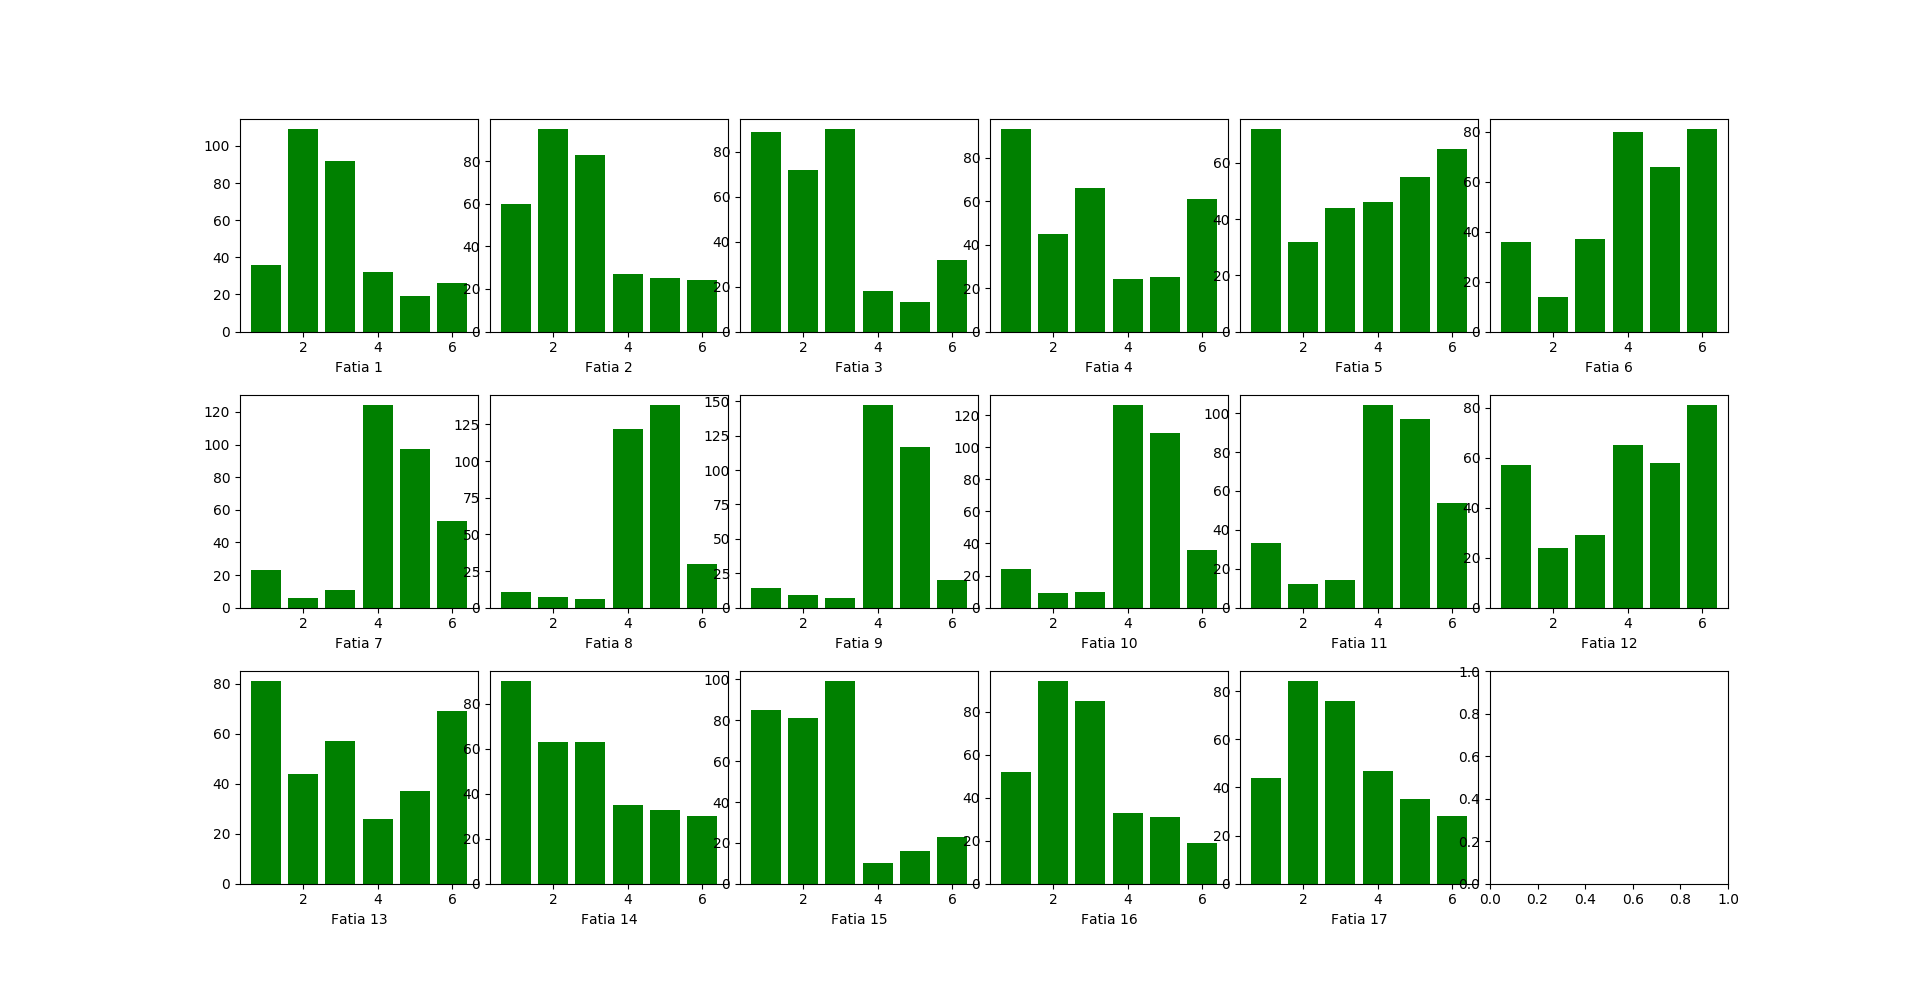
\includegraphics[width=2.5in]{imgs/antes_shuffle}
\caption{Distribuição dos dados antes do shuffle}
\label{fig:antes_shuffle}
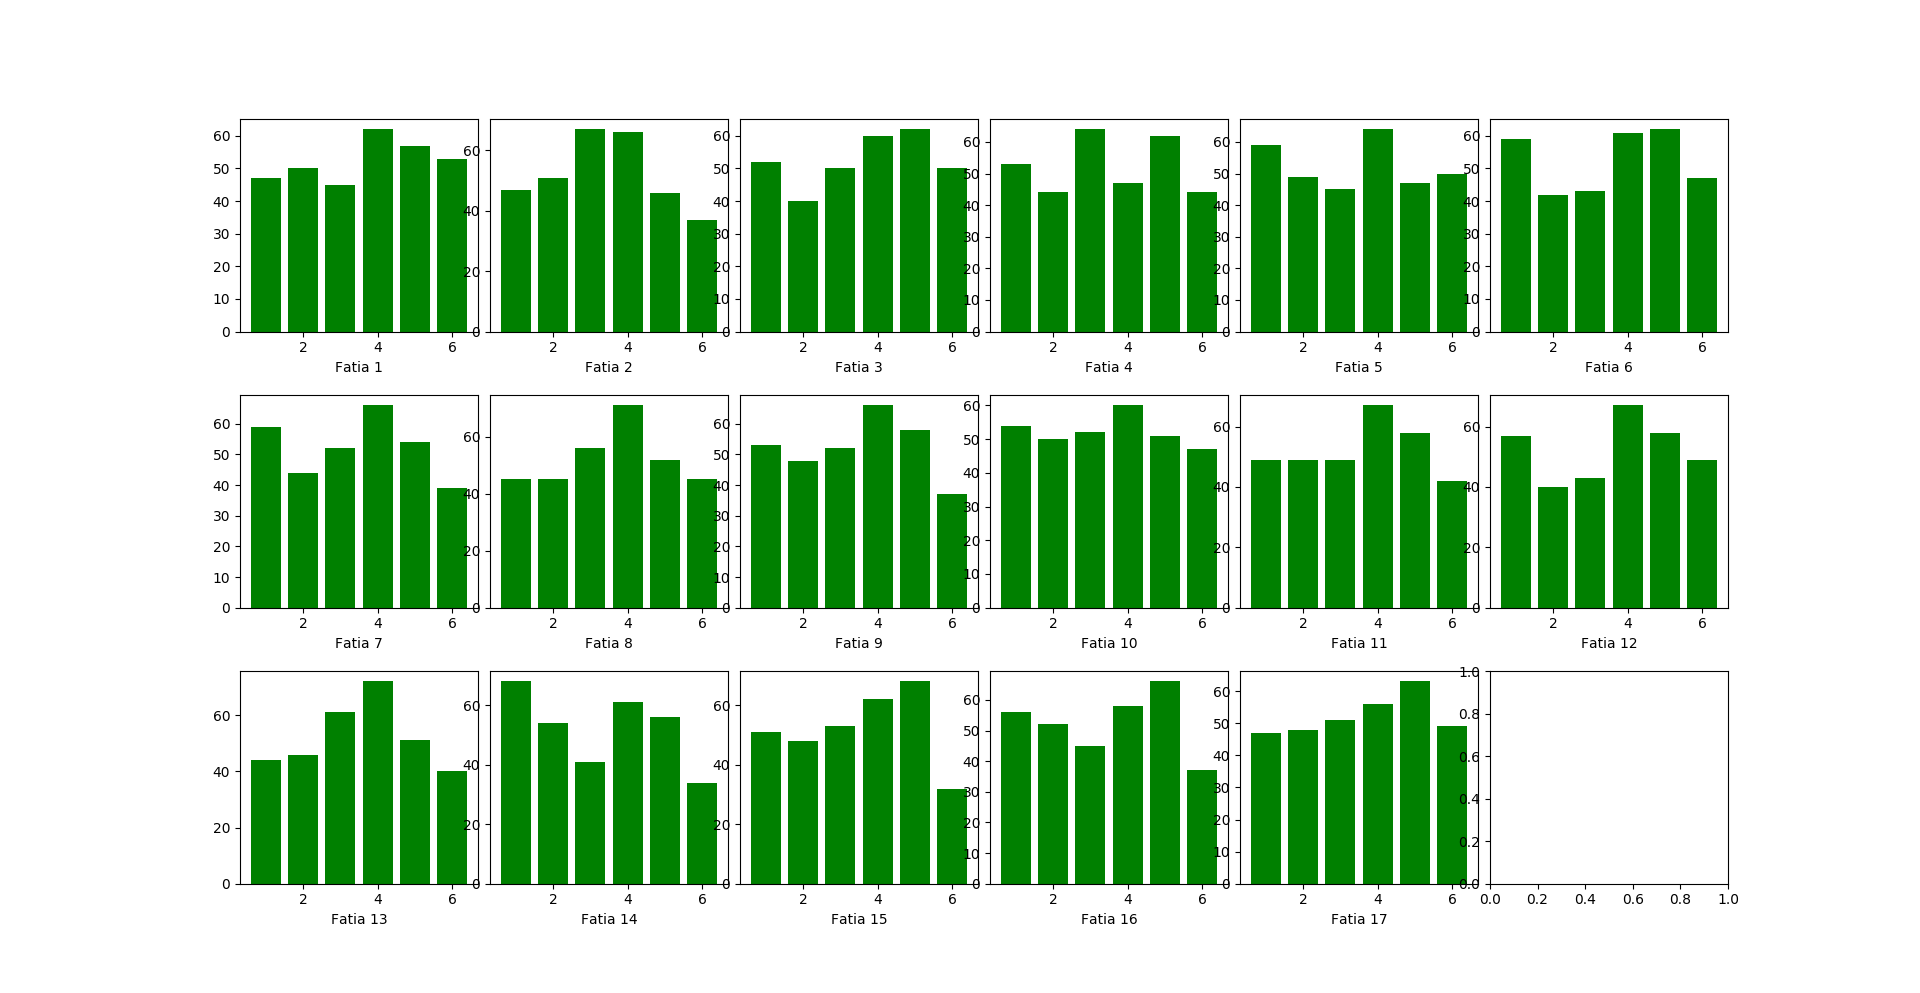
\includegraphics[width=2.5in]{imgs/apos_shuffle}
\caption{Distribuição dos dados depois do shuffle}
\label{fig:apos_shuffle}
\end{figure}

\section{Metodologia Experimental}\label{sec:metodologia}
\subsection{Sistema de Avaliação}\label{subsec:sistema_avaliacao}
%Divisões entre treinamento e teste
A fim de conseguir avaliar o desempenho de predição dos diferentes modelos 
de Aprendizado de Máquina sobre a base de dados fornecida, decidimos utilizar 
a técnica de \textit{10-Fold Cross Validation} que é ideal para adequar os 
dados de treinamento e teste. Para isso, dividimos a quantidade total de 
amostras por $10$ e portanto, teremos $10$ \textit{folds} (fatias) dos dados 
com tamanhos iguais. Para cada fatia N indo de $1$ a $10$, deixamos a atual 
sendo utilizada para uma partição de teste e o restante é utilizado como partição 
de treinamento, semelhante ao descrito em \cite{cross_validation}. Se uma partição de 
teste não fosse utilizada para a definição dos parâmetros, possivelmente 
teríamos um valor de F-medida máximo gerado por \textit{overfitting} da própria 
partição de treinamento. Analogamente, deixar mais \textit{folds} para teste e
menos para treinamento faria com que a capacidade de generalização dos modelos
pudesse ser melhor avaliada, mas em contrapartida menos dados seriam usados para
a hipótese, o que poderia diminuir sua F-medida consideravelmente.


Além disso, para que conseguíssemos otimizar a validação cruzada juntamente 
com a estimativa de parâmetros mais adequados para os algoritmos, utilizamos 
o \textit{Grid Search}. Basicamente o que fazemos em todo o processo é escolher 
o valor do parâmetro que apresenta a maior F-medida para cada uma das partições 
utilizadas para teste na validação cruzada. Assim, é possível analisar todos os
resultados e escolher o \textit{fold} que melhor otimiza todos os modelos 
utilizados no projeto através de uma média das F-medidas. Desta forma, podemos
então escolher o algoritmo que apresenta os melhores resultados para a base de
dados descrita na seção~\ref{sec:base_dados}.

Para o treinamento de algoritmos mais custosos como Redes Neurais Artificiais 
e o SVM, consideramos necessária a redução da grande quantidade inicial de 
atributos. Para isso, foi feita a matriz de correlação entre os atributos, onde
colunas da matriz cuja correlação era maior que $0.9$, menor que $-0.9$ foram 
removidas. Resultando em $170$ atributos aproximadamente de um total de $561$. 
Apesar da redução ter sido significativa, esse número ainda resultaria em 
execuções custosas para a geração de hipóteses. Posto isso, após algumas 
pesquisas e conselhos, o grupo decidiu fazer a implementação do método de 
Análise de Componentes Principais, disponível no arquivo \texttt{pca.m}, optando por manter atributos que preservam 
no mínimo $98\%$ da variância dos dados apresentados inicialmente, de maneira 
que a fidelidade das informações se mantivesse. Após feito o processo em cima 
da base de dados já normalizada, restaram $151$ atributos.


\subsection{Parâmetros e Medidas de Desempenho}
%Descrever as decisões do grupo nos que foram utilizados
Para o classificador KNN precisávamos definir uma maneira eficiente para 
encontrar o número ideal k de vizinhos para assim determinar a distância entre 
os pares. Para isso, capturamos o k, indo de 1 a 50, que atribui a melhor 
F-medida de predição ao KNN utilizando as partições de treinamento e teste 
definidos pelo \textit{10-Fold Cross Validation}. Para a implementação do 
K-vizinhos mais próximos utilizamos vetorização em vários passos, de forma a melhorar o desempenho da execução.

A Regressão Logística contou com a variação apenas do parâmetro lambda, sendo
esta de $0$ a $10$. Isso
ocorreu principalmente pela grande quantidade de atributos usados, o que tornou
inviável a geração de atributos polinomiais. 


Para os algoritmos de Redes Neurais Artificiais existem vários parâmetros que
influenciam diretamente no funcionamento do algoritmo. O grupo optou por testar
as variações de lambda, número máximo de iterações e número de neurônios das
camadas ocultas. 

O parâmetro de maior dificuldade para definição foi o número de
neurônios das camadas ocultas porque impactava diretamente o tempo de
processamento e a qualidade de resultado. Para isso, o grupo buscou por
materiais e conselhos que pudessem ajudar e, a partir disso, definimos três
variações de neurônios: 
    \begin{description}
        \item[75]{Aproximadamente metade dos atributos. Esperava-se que a
        acurácia para este parâmetro fosse mais baixa.}
        \item[151]{Iguala o número de atributos depois da aplicação da Análise
        de Componentes Principais.}
        \item[300]{Esperava-se que este parâmetro, combinado com o lambda certo,
        resultasse na melhor acurácia possível apesar do alto cuso
        computacional}
    \end{description}

Para as RNA de apenas uma camada, o número máximo de iterações variou entre 200,
500 e 700. Já para as de duas camadas, este parâmetro variou entre 500, 750 e
1000.

A variação do lambda foi também um ponto de dificuldade para o caso específico
de lambda igual a 0. Isso ocorreu porque, entre os cálculos do método, o custo
acabava se tornando um NaN (Not a Number) e fazia com que o método divergisse.
Para corrigir este problema, implementou-se uma verificação que, sempre que o
cálculo do custo resultasse em um NaN, era adicionado um número suficientemente
próximo de zero ao valor, desssa forma tornando possível a computação sem
maiores problemas.

Devido a grande quantidade de funções de Kernel e diferentes parâmetros para a
técnica de classificação de Máquinas de Vetores de Suporte, foram escolhidos
parâmetros que mais sintetizam nosso conjunto de dados. Primeiramente, para
montar o \textit{grid} com os valores ótimos para cada \textit{fold} da técnica 
de \textit{10-Fold Cross Validation}, iteramos os parâmetros C (responsável 
pela largura da margem) e Gamma (Parâmetro do \textit{kernel} RBF,
\textit{Radial Basis Function}) exponencialmente.

Para o parâmetro C, a iteração ocorreu dos valores: $2^{-3}$ até $2^4$. Valores 
maiores que isso ultrapassaram o número máximo de iterações da função svmtrain. 
Para o parâmetro Gamma do kernel RBF, o alcance foi entre $2^{-15}$ até $2^3$.
Também, além de utilizarmos o \textit{Kernel} RBF para montar o \textit{grid}, 
montamos um \textit{grid} separado para visualizar como o SVM se comportaria 
com um \textit{Kernel} linear, e após constatarmos que a nossa base dados não 
é linear, e analisarmos o \textit{grid} resultante, descartamos este método 
de classificação, por sua F-medida ser inferior a todos os outros métodos.

Como foi descrito anteriormente, o \textit{grid} com os valores ótimos para cada K da
técnica de \textit{K-Fold} precisavam de dois parâmetros, C e Gamma, tornando o \textit{grid} de
três dimensões. Para contornar esta dificuldade que dificultaria a visualização 
dos dados, montamos a matriz com dimensões de 10 x 190, onde 10 representa a 
técnica de \textit{10-Fold Cross Validation}, e 190 representa as 10 iterações possíveis 
de C multiplicadas por 19 iterações possíveis de Gamma. Com isso, cada coluna 
seria uma combinação possível de valores de C e Gamma, mantendo sua visualização em duas dimensões.



\section{Resultados}\label{sec:resultados}
%Colocar muitas tabelas e gráficos de comparação para mostrar os resultados de predição de cada algoritmo
De acordo com a estrutura do nosso \textit{grid}, primeiramente recuperamos os valores 
de parâmetros, descritos na seção \ref{sec:metodologia}, que apresentam melhor 
F-medida para cada \textit{fold} da validação cruzada. As melhores F-medidas resultantes 
deste processo podem ser visualizadas na tabela \ref{fmedidas}. Como pode 
ser conferido, a melhor F-medida média foi detectada para o \textit{fold} 4 e 
portanto, estabelecemos que esse é o \textit{fold} ideal para todos os modelos. A partir 
disso, podemos utilizar os melhores valores dos parâmetros de cada modelo em 
relação ao \textit{fold} 4. Os parâmetros definidos podem ser visualizados na tabela
\ref{parametros}. É necessário salientar que para redes neurais, talvez a 
qualidade seja afetada positivamente ou negativamente, pois os pesos para o 
cálculo dos neurônios é totalmente aleatório em cada execução.

\begin{table}[!t]
% increase table row spacing, adjust to taste
\renewcommand{\arraystretch}{1.3}
\caption{Melhores F-medidas (em \%) dos modelos para cada \textit{fold}}
\label{fmedidas}
\centering
% Some packages, such as MDW tools, offer better commands for making tables
% than the plain LaTeX2e tabular which is used here.
    \begin{tabular}{|l|c|c|p{0.9cm}|p{0.9cm}|c|p{0.8cm}|}
    \hline
    & KNN & RL & RNA 1 camada & RNA 2
    camadas & SVM & F-medida média\\
    \hline
    Fold-1 & 94.724 & 88.494 & 91.490 & 91.550 & 92.608 & 91.773 \\ 
    Fold-2 & 94.143 & 86.479 & 90.448 & 89.761 & 92.482 & 90.662 \\
    Fold-3 & 93.295 & 86.614 & 91.124 & 90.591 & 92.418 & 90.808 \\ 
    Fold-4 & 94.210 & 89.510 & 92.937 & 94.333 & 96.104 & 93.418 \\ 
    Fold-5 & 93.806 & 87.193 & 92.426 & 93.165 & 93.573 & 92.326 \\ 
    Fold-6 & 94.773 & 86.931 & 92.275 & 92.108 & 93.839 & 91.985 \\ 
    Fold-7 & 95.132 & 86.979 & 92.024 & 93.397 & 92.495 & 92.005 \\ 
    Fold-8 & 92.573 & 84.634 & 91.218 & 92.393 & 92.976 & 90.758 \\ 
    Fold-9 & 94.307 & 85.959 & 91.222 & 91.613 & 93.750 & 91.370 \\ 
    Fold-10 & 94.010 & 89.633 & 91.750 & 92.425 & 93.455 & 92.255 \\
    \hline
    \end{tabular}
\end{table}


Após feita a seleção dos melhores parâmetros para cada classificador como foi 
descrito anteriormente, fizemos uma análise do desempenho de cada um dos 
algoritmos através das seguintes métricas: F-medida, precisão, revocação, 
acurácia e por fim, tempo de execução. A precisão e a revocação que geraram 
os F-medidas, foi uma realizada através da média da precisão e revocação de 
todas as classes, já que temos seis. Nossos dados estão poucos desbalanceados, 
como vimos do pré-processamento, então a acurácia possivelmente também 
representa valores, que em sua maioria, são verídicos. O tempo de execução 
no Octave foi recuperado através dos comandos complementares tic() e toc(), 
que disparam um timer no início da execução do algoritmo e registram o tempo 

total no final \cite{octave:tictoc}. O tempo de execução é sensível à infraestrutura onde os algoritmos serão executados. No nosso caso, utilizamos um computador equipado com 16GB de Ram DDR3 e um processador Intel i7 para realizar o \textit{grid search} e para a execução dos parâmetros já otimizados, utilizamos um notebook equipado com 8GB de Ram DDR4 e processador Intel i7.
Todos esses valores podem ser visualizados de forma mais 
representativa na tabela \ref{metrica_otimos}.

\begin{table}[]
\centering
\caption{Valores ótimos dos parâmetros definidos pelo \textit{grid} para cada modelo}
\label{parametros}
\begin{tabular}{|l|l|l|}
\hline
Modelo                                              & \multicolumn{1}{|l|}{Parâmetro} & Valor     \\ \hline
KNN                                                 & K                              & 1         \\ \hline
RL                                                  & Lambda                         & 2         \\ \hline
\multicolumn{1}{|c|}{\multirow{3}{*}{RNA 1 Camada}} & Iter                           & 750       \\
\multicolumn{1}{|c|}{}                              & Lambda                         & 1         \\
\multicolumn{1}{|c|}{}                              & Neurônios                      & 151       \\ \hline
\multirow{3}{*}{RNA 2 Camadas}                      & Iter                           & 1000      \\
                                                    & Lambda                         & 2         \\
                                                    & Neurônios                      & 300       \\ \hline
\multirow{2}{*}{SVM}                                & C
& 16        \\
                                                    & Gamma                          & 0.0078125 \\ \hline
\end{tabular}
\end{table}

\begin{table}[!t]
% increase table row spacing, adjust to taste
\renewcommand{\arraystretch}{1.3}
\caption{Métrica dos classificadores utilizando os parâmetros ótimos}
\label{metrica_otimos}
\centering
\begin{tabular}{|p{1.8cm}|c|c|p{1cm}|p{1cm}|c|}
\hline
    & KNN & RL & RNA 1 camada & RNA 2
    camadas & SVM\\
\hline
F-medida (\%) & 94.210 & 89.141 & 91.997 & 93.501 & 95.521 \\
Precisão (\%) & 94.060 & 89.126 & 91.813 & 93.320 & 95.346 \\
Revocação (\%) & 94.360 & 89.156 & 92.183 & 93.684 & 95.696 \\
Acurácia (\%) & 93.996 & 88.930 & 91.932 & 93.433 & 95.497 \\
Tempo de Execução (em segundos) & 59.924 & 14.660 & 208.183 & 1025.951 & 10.029 \\
\hline
\end{tabular}
\end{table}

Além disso, geramos as curvas de aprendizado para cada um dos métodos para
mensurar o que há ou não de errado e poder refletir a respeito de medidas de
correção para aumentar o desempenho de cada método. 

Para o KNN, não faria sentido gerar uma curva conforme o erro de predição do conjunto de treinamento com k = 1, uma vez que todas as amostras seriam conhecidas. Desta forma, utilizamos o k = 2 que é o segundo parâmetro que demonstrou uma melhor F-medida (aproximadamente 93\%) para o fold selecionado. O gráfico gerado para k = 2 pode ser visto na figura \ref{fig:knn_curve}.
O gráfico de todos os outros algoritmos foi gerado com os parâmetros ótimos encontrados anteriormente. Apesar disso podemos analisar através das imagens que, todos com exceção da Regressão Logística (figura \ref{fig:rl_curve}), demonstraram um super-ajustamento pertinente. O super-ajustamento pode ser explicado por vários fatores como, por exemplo, modelos muito complexos para uma base dados pequena, amostras com baixas variâncias e etc.

\begin{figure}[!t]
\centering
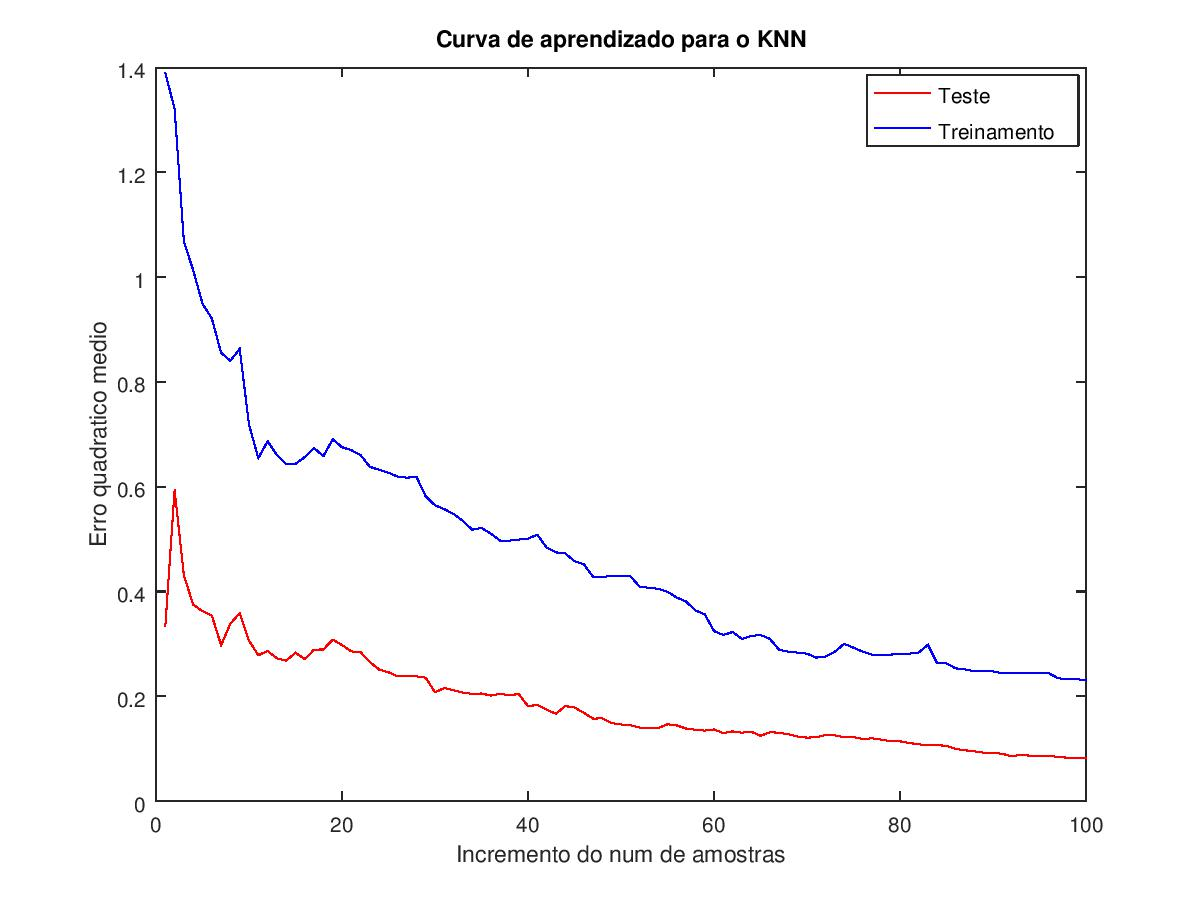
\includegraphics[width=3.5in]{imgs/KNNk2Curve.jpg}
\caption{Curva de Aprendizado para o método KNN com k = 2}
\label{fig:knn_curve}
\end{figure}

\begin{figure}[!t]
\centering
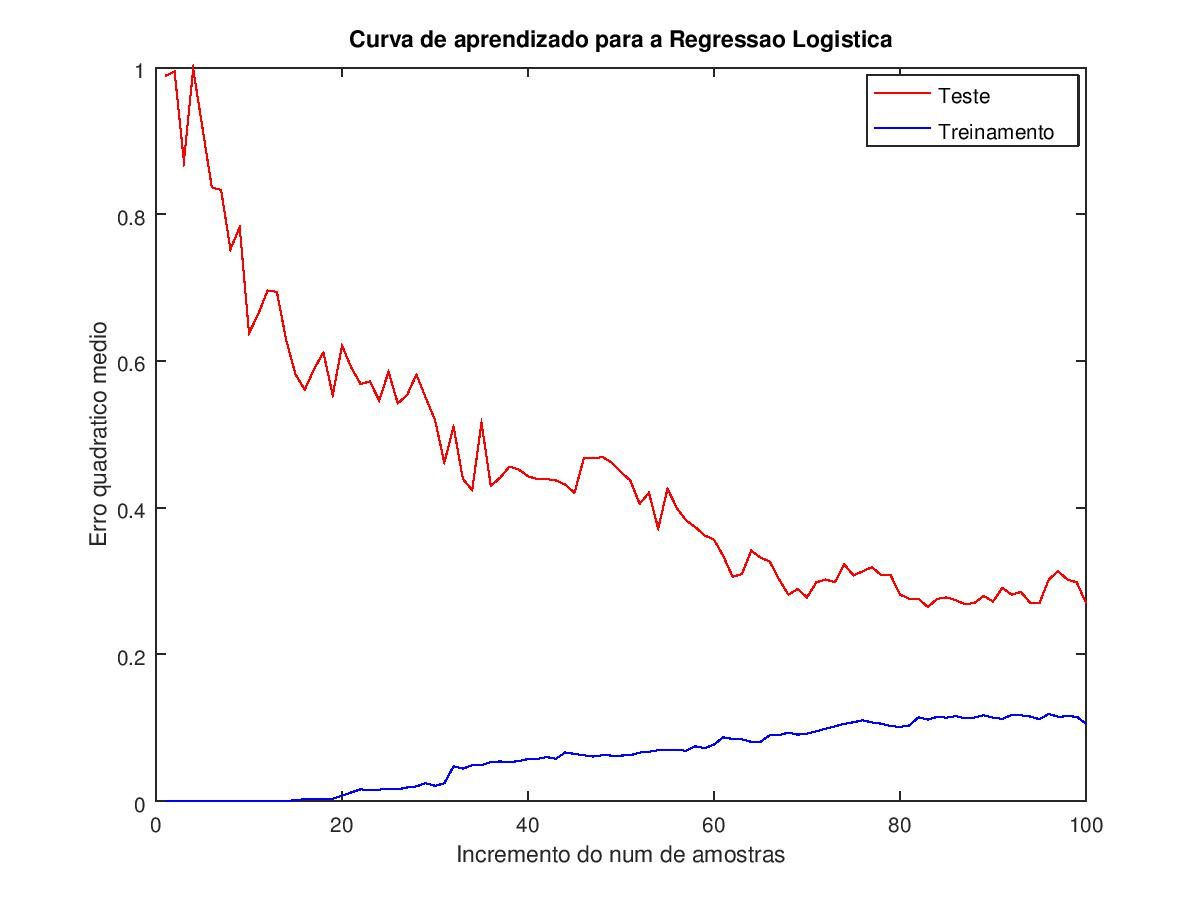
\includegraphics[width=3.5in]{imgs/RLcurve.jpg}
\caption{Curva de Aprendizado para o método de Regressão Logística}
\label{fig:rl_curve}
\end{figure}

\begin{figure}[!t]
\centering
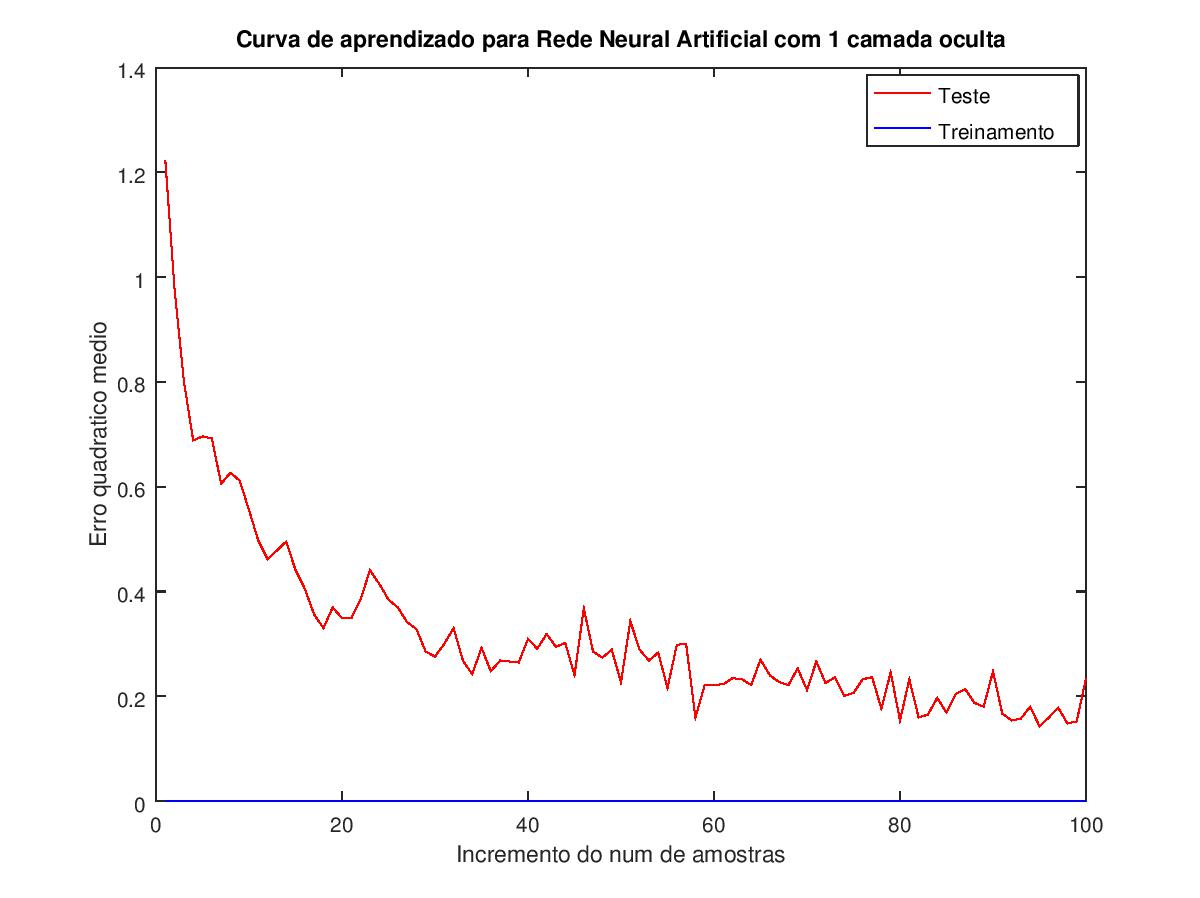
\includegraphics[width=3.5in]{imgs/RN1Curve.jpg}
\caption{Curva de Aprendizado para o método de Redes Neurais Artificial com 1 camada oculta}
\label{fig:rn1_curve}
\end{figure}

\begin{figure}[!t]
\centering
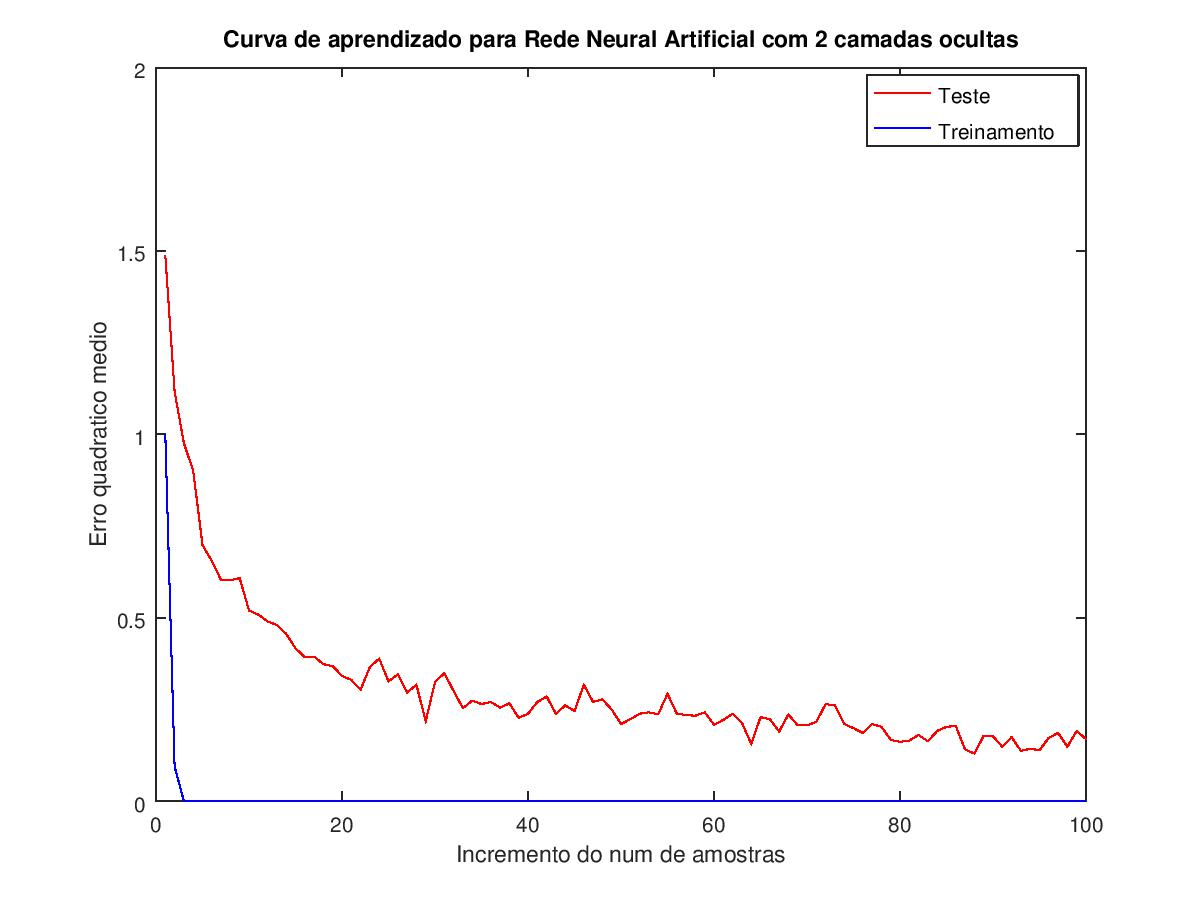
\includegraphics[width=3.5in]{imgs/RN2Curve.jpg}
\caption{Curva de Aprendizado para o método de Redes Neurais Artificial com 2 camadas ocultas}
\label{fig:rn2_curve}
\end{figure}

\begin{figure}[!t]
\centering
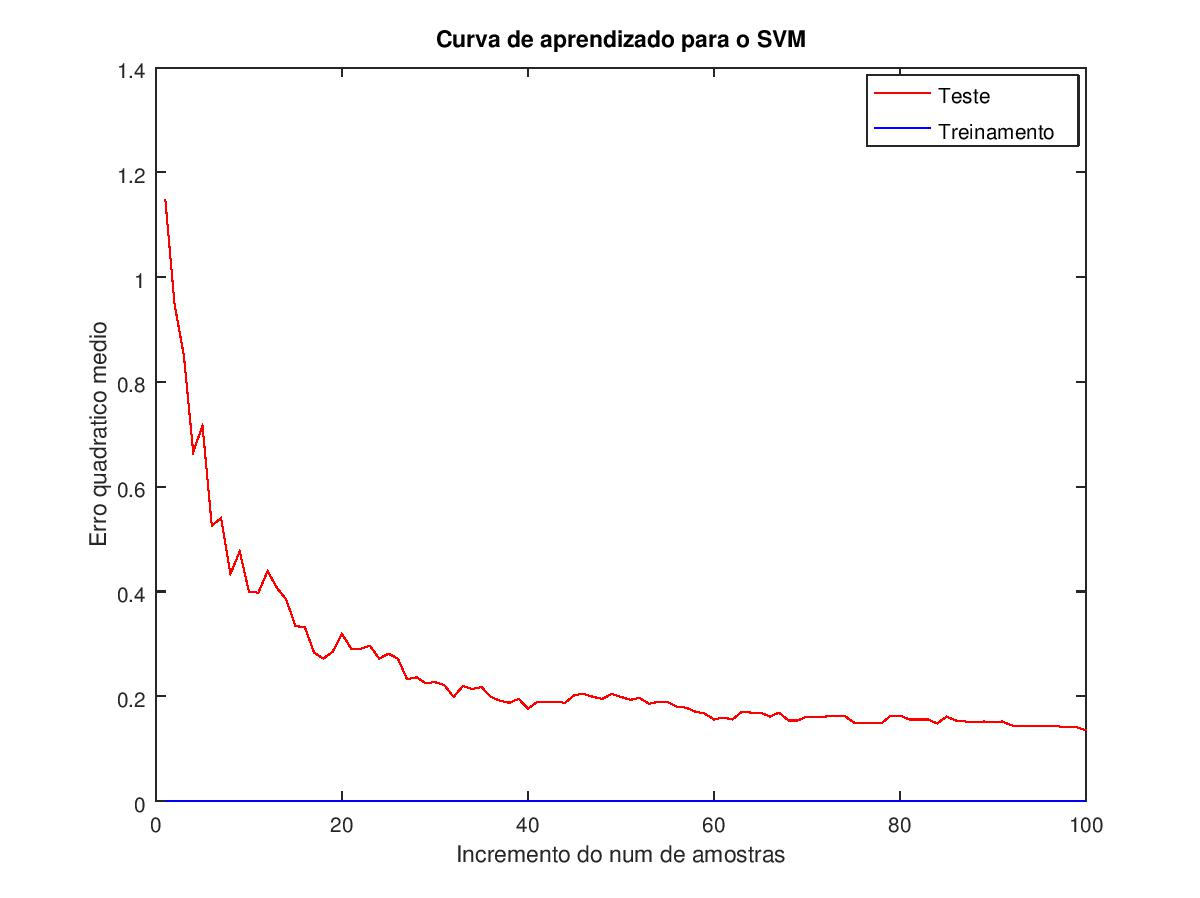
\includegraphics[width=3.5in]{imgs/SVMcurve.jpg}
\caption{Curva de Aprendizado para o método SVM}
\label{fig:svm_curve}
\end{figure}

Para o KNN, uma possível solução para contornar o super-ajustamento seria testar
outras medidas de dissimilaridade em combinação com K maiores. Já para a
Regressão Logística, a literatura recomenda como uma solução para reduzir o
super-ajustamento reduzir a complexidade do modelo, deixando o classificador
mais linear, porém no nosso caso, não acrescentamos nenhum polinômio derivado,
sendo necessário recorrer à modificações e/ou reduções nos atributos da base de
dados. Se tratando de Redes Neurais Artificiais, por outro lado, uma maneira de
evitar o super-ajustamento seria empregar a técnica de \textit{Dropout}, onde
nela, podemos iterar um certo número de vezes a rede neural, desativando alguns
pesos randomicamente e observando a eficácia de predição. Após isso, basta
eleger o modelo ``magro''  de desempenho satisfatório. 
Por fim, para o SVM, temos que o \textit{overfitting} pode ser amenizado através 
da utilização do \textit{kernel} linear ao invés de um \textit{kernel} Gaussiano, 
por exemplo, uma vez que o número de amostras não é grande e a utilização do 
\textit{kernel} Gaussiano tende a tornar o modelo muito complexo \cite{svm_user_guide}. 
Neste caso em específico, como estamos utilizando o \textit{kernel} RBF, a melhor 
decisão seria tentar reduzir o tamanho do parâmetro C e aumentar o valor do 
parâmetro Gamma \cite{svm_quora}.

\section{Conclusões}\label{sec:conclusao}
Antes de mais nada, gostaríamos de frisar a importância do pré-processamento no aprendizado de máquina, pois sem ele, ou com sua aplicação de forma errônea, a porcentagem de acerto do modelo final vem a ser bem baixa.

    Em seguida, o processo de tuning dos algoritmos através da formação do \textit{grid search} é computacionalmente exaustivo, porém completamente necessário para que se encontre os parâmetros ótimos para a geração de um bom modelo. Infelizmente, mesmo com todos os processos realizados, presenciamos a geração de overfitting em vários modelos quando comparados com a base de treinamento, ou seja, com amostras já conhecidas. Acreditamos que um dataset com mais amostras pudesse reduzir a variância dos erros e otimizar de maneira mais precisa a classificação, porém este passo não estava ao nosso alcance neste projeto.
    
    Por fim, após o grupo gerar as hipóteses com diferentes algoritmos de
aprendizado, pode-se observar que especificamente para essa base de dados, o
modelo criado pela Máquina de Vetores de Suporte conseguiu gerar o melhor modelo
de predição, resultando em uma F-medida média de 95.5\% na classificação das
amostras de teste. De maneira geral, nosso resultado foi satisfatório. Como
citado por \cite{guia_svm}, que apresenta a aplicação do SVM em uma base muito próxima à utilizada neste projeto e que utilizou um pré-processamento mais simples, a performance do SVM na base de teste ficou entre 90\% e 96\%.


% referências
\printbibliography


\appendix
\section{Execução do projeto}\label{apendice_execucao}
%Passo-a-passo para obter os resultados no Octave que foram detalhados no relatório
Para que a execução do projeto ocorra de forma ideal, é necessário que a 
hierarquia de pasta de todos os arquivos anexados seja mantida da maneira em que fora 
entregue, sem mudanças de diretório.

É necessário também que haja a biblioteca libsvm para a execução do algoritmo 
de máquina de vetores de suporte, o projeto já fornece a biblioteca compilada 
para o sistema operacional Windows (32/64bits) e para o Linux (64bits). 
Caso pretenda executar em um sistema operacional diferente, será necessário 
compilar e adicionar a biblioteca ao path do Octave/Matlab antes de executar o 
projeto, para mais informações, o link do repositório se encontra em
\cite{libsvm}

Além da biblioteca para o algoritmo SVM, ainda em trechos de código de Redes 
Neurais Artificiais, utilizamos dos pacotes io e statistics do próprio Octave. 
Para o cálculo dos erros quadráticos e o plot dos gráficos de curvas de 
aprendizado também fazemos uso do pacote image do Octave. É necessário que 
seja feita a instalação dos mesmos da maneira que é descrito em
\cite{octave:install_remove}. 

Inicialmente, fornecemos os dados com um pré-processamento já aplicado que 
foram gerados e gravados no arquivo de nome \texttt{pre\_processed.mat}. Porém, se por 
algum motivo for necessário fazer o pré-processamento novamente, é necessário 
executar no Octave/Matlab o arquivo preprocessing.m que utiliza os arquivos da 
base de dados inicial fornecidos no diretório dataset\_uci. Vale a pena 
ressaltar que toda vez que o pré-processamento é executado, ocorre um novo 
shuffle nos dados, tal qual pode alterar razoavelmente os resultados aqui apresentados.

Para visualizar e/ou executar os testes feitos pelo grupo com a formação do 
\textit{grid} search e \textit{10-fold cross validation}, é necessário que seja feita a execução 
do arquivo \texttt{exec\_project.m}. É importante alertar que a execução deste arquivo 
completo pode vir a demorar mais de 24h por se tratar de um código que passa 
por muitas iterações.

Para visualizar e/ou executar o resultado dos classificadores com os parâmetros
ótimos já selecionados, de maneira a entender a qualidade apresentada por cada 
um através da F-medida, é necessário que seja feita a execução do arquivo 
\texttt{optimized\_project.m}.
A geração das curvas de aprendizado como descritas na seção
\ref{sec:resultados} estão contidas no arquivo \texttt{learning\_curves.m}.


% that's all folks
\end{document}
